\section{Conflicts}\label{ssec:conflicts}
As mentioned back in \cref{ch:uppaalmodel}, we did not enforce the physical rules of modules to the fullest. These entail that a module may not connect to another module if this module is not a neighbour and if the connection would force two modules to take up the same space. The anti-serialization transformations rules can currently create configurations in which not all modules are connected to neighbours, and this problem will be solved in \cref{ssec:restrictbranch}. Furthermore both our anti-serialization and parallelization rules can cause intersections to occur, and we will solve this problem in \cref{ssec:paround} and \cref{ssec:pbeneath}.


\subsection{Restricting Branches Anti-Serialization}\label{ssec:restrictbranch}
For the anti-serialization transformation rules described in \cref{sec:as} we did not make sure that when we connected new lines to the main line, that the start and end of these lines were neighbours to the first and last module of the line. Furthermore, untill now, we have imagined that no other branch has been made from our line when performing the transformation. Yet, this will not always be the case, and as such can cause some conflicts.

\subsubsection{Neighbour Errors}
Imagine a situation similar to what the rule $AS_0$ in \cref{fig:as0} describes. Here we have specific $s$ and $e$ modules chosen on a line $\gamma$ and we have chosen to branch out a specific recipe $r$. Between the two modules we have $M_{s,e}$. From this we can calculate $A_{r,s,e}$ and $B_{r,s,e}$ as described before. If $0 < |B_{r,s,e}|$, then we may branch out some modules only used to work on $r$. However in  most cases $B_{r,s,e}$ will not have a size such that it can be connected in reality to the $s$ and $e$ modules. We therefor modify our $AS_0$ transformation rule so that solves this.

If $|A_{r,s,e}| + 2 > |B_{r,s,e}|$ , then the result of our $AS_0$ transformation rule will be the top of \cref{fig:astrans}. In this case we append the new line with transport modules to make the two lines fit each other. Notice that the modules beneath the new line are marked as shadowed, i.e. coloured red. This is used in order to handle transformation conflicts as described below in Shadowed Modules. We also introduce blue rounded boxes with indexes to the top right of them. These boxes mean that anything inside of them are serialized $i$ times, where $i$ is the index given with the box. 


If $|A_{r,s,e}| + 2 \leq |B_{r,s,e}|$,  then the result of our $AS_0$ transformation rule will be the bottom of \cref{fig:astrans}, In this case we append the original line with transporters instead of the new line to make them fit together.

\begin{figure}[H]
	\centering
	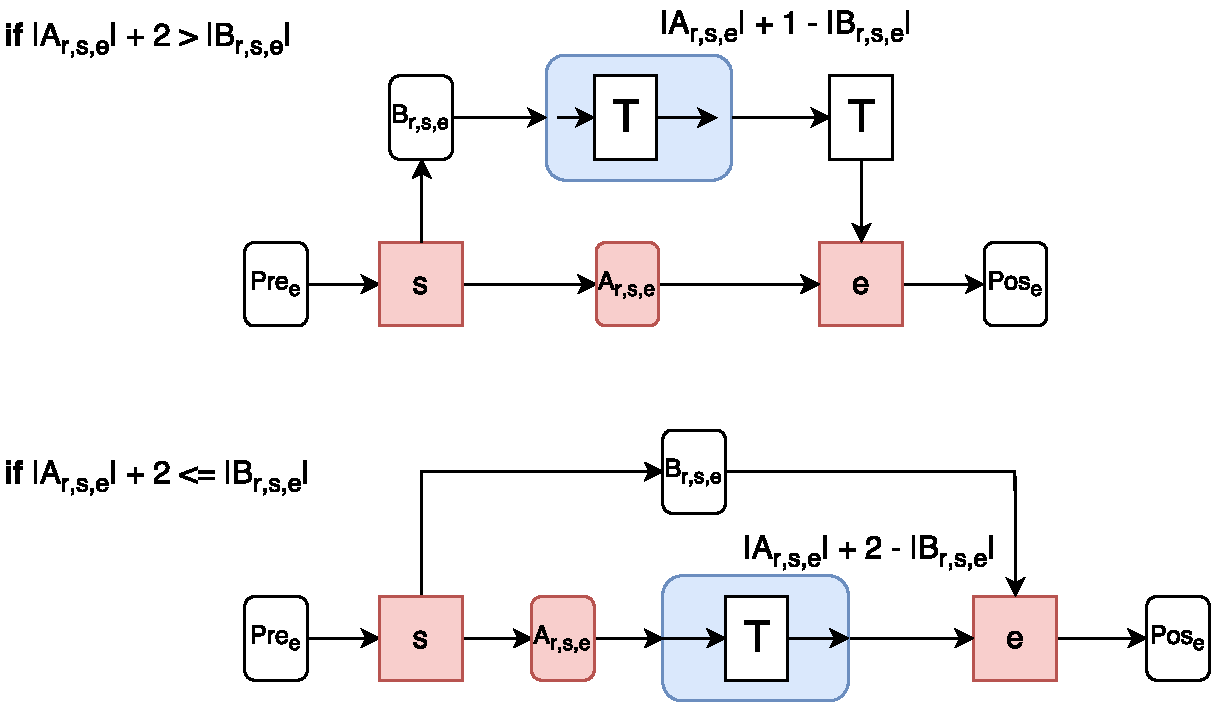
\includegraphics[width=\textwidth]{astrans.pdf}
	\caption{The new results of $AS_0$}
	\label{fig:astrans}
\end{figure}

\subsubsection{Shadowed Modules}
On the top part of \cref{fig:shadowexample}, we see that we have already made a branch from $s1$ to $e1$, which results in the modules on the other line being shadowed. Being shadowed means that if we remove the module and just reconnect the old line as usual, then the branch becomes too long to connect back to its old line, and shadowed boxes are visualized with the colour red. The line needs to connect back to its designated point on the old line as the module located here is a common module. It performs work on the recipe $r$ otherwise worked on by the new line and should therefore not be bypassed.  To get around this we, as shown in \cref{fig:shadowexample}, alter our anti-serialization transformation in this case to replace a shadowed module with a transport module, as not to skew the two previous lines away from each other. The example shows this done for a single module, but it may be done regardless of the amount of shadowed modules which we remove. In \cref{fig:shadowexample} we also introduce rounded boxes with three dots in them. These boxes just means any number of modules in a total order.

We may however not do this if the shadowed module is also a module where a branch either connects from or to. This means that the module is common and is used by the branch. Removing it would keep us from producing that branch's specific recipe. Therefore we never allow for these modules to be removed, even if this means that we can not perform certain anti-serializations.

\begin{figure}[H]
	\centering
	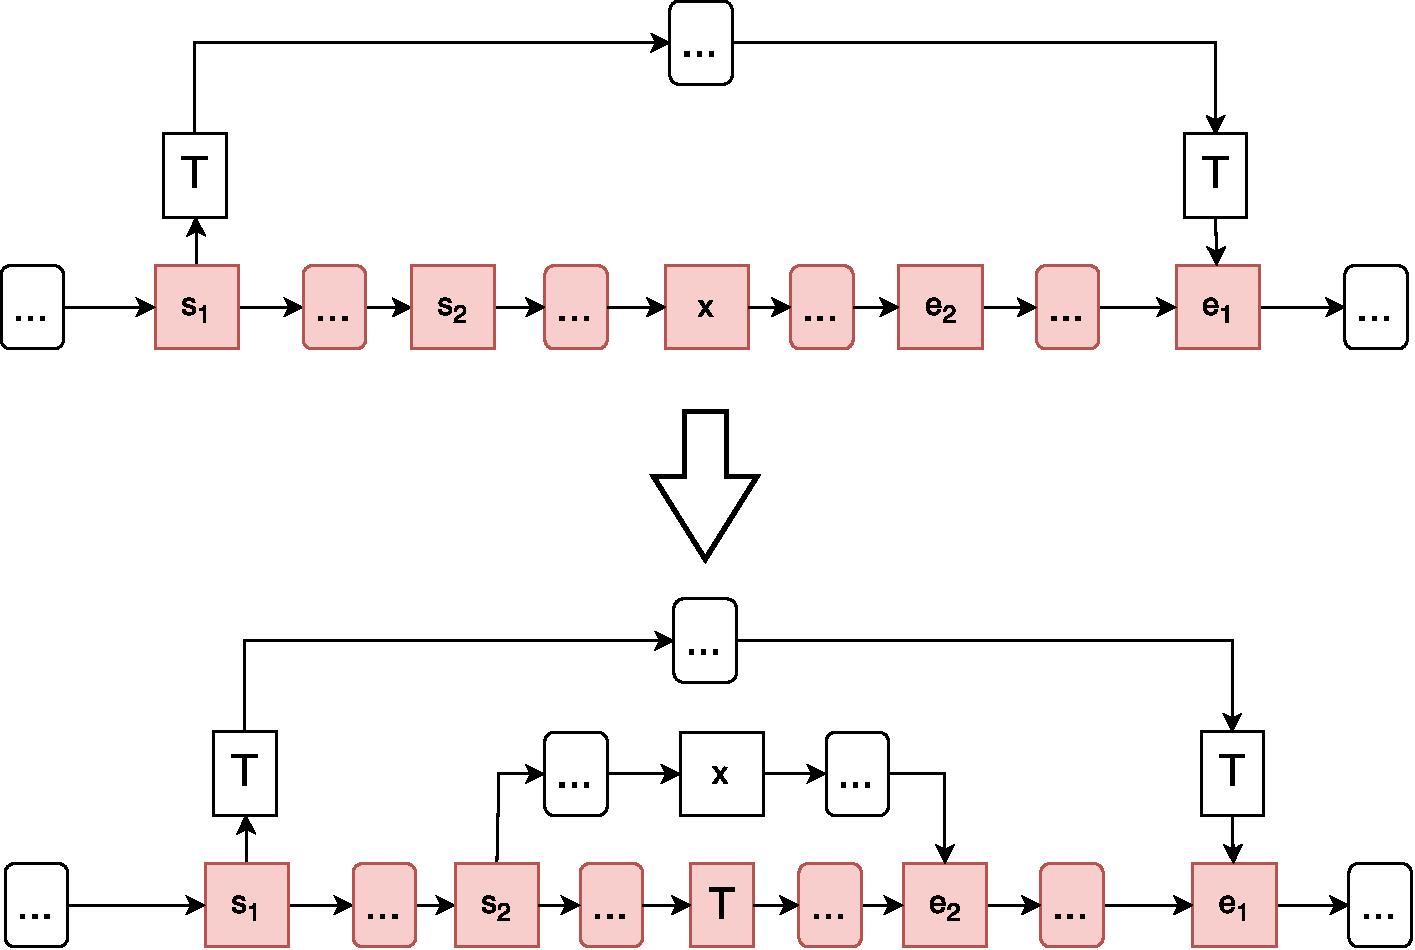
\includegraphics[width=\textwidth]{as5.pdf}
	\caption{Transformation that handles the case where an anti-serialization removes a shadowed module}
	\label{fig:shadowexample}
\end{figure}

\subsection{Push Around} \label{ssec:paround}
In push around we handle the case where a new off branching line intersects with an old line, by moving the new line above the old line. In the case where the new line entirely covers the old we perform the transformation depicted in \cref{fig:pusharound1}. As shown, the new line simply uses transport modules to lift itself up above the old line. These transport modules are technically not a part of the line and only serve the purpose of avoiding the intersection.

\begin{figure}[h]
\centering
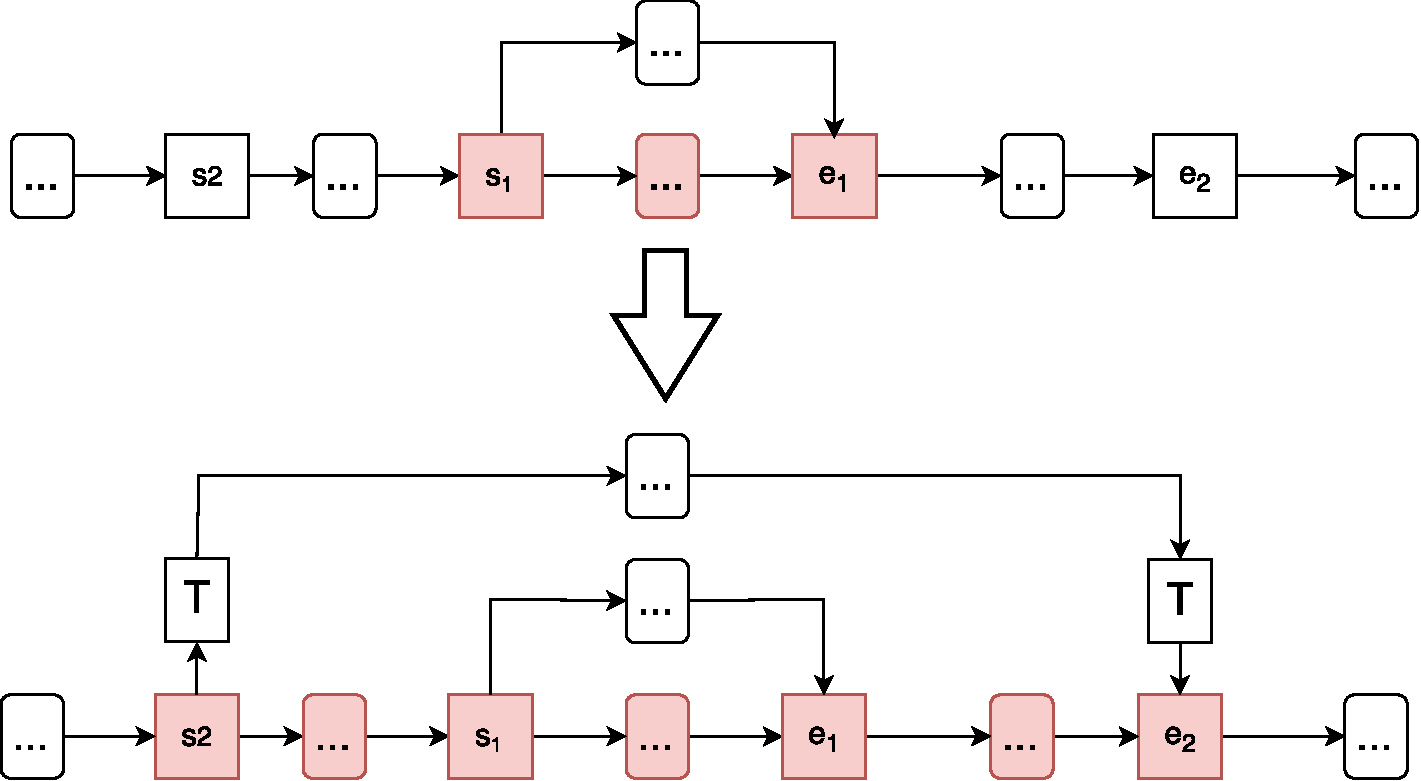
\includegraphics[width=\textwidth]{conflict1.pdf}
\caption{How push around handles the case, where we insert a new line that covers the entirety of an old line}
\label{fig:pusharound1}
\end{figure}

There is also the case where the new line is covered by the old line entirely. In this case we use the transformation in \cref{fig:pusharound2}. Here we do not need to append any transport module as we move up through the already existing modules, which we would otherwise intersect with. 

In the cases where the new entirely intersects the old it will add transport modules where needed, or otherwise guide itself vertically through modules that already exists. These examples only show the case, where a single old line is placed above the main line from which we branch off. In the case of more line levels, the new line will simply climb vertically until it finds a level where it may be placed without intersection. 

Push around is the intersect handling we use when inserting new lines as a result of anti-serialization, as there is no need to keep this new line close to the one from which it sprouted. 

\begin{figure}[H]
\centering
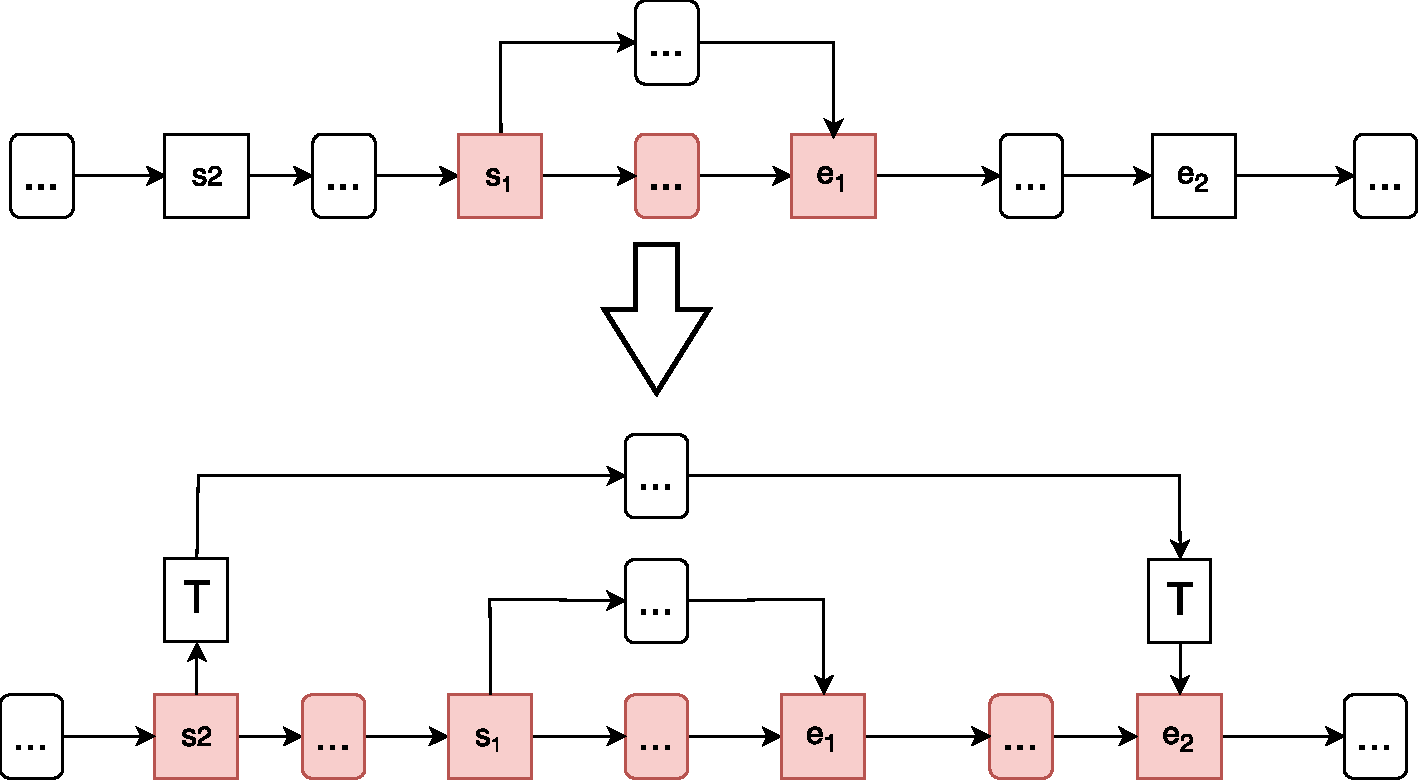
\includegraphics[width=\textwidth]{conflict2.pdf}
\caption{How push around handles the case where we insert a new line that is covered by the entirety of an old line}
\label{fig:pusharound2}
\end{figure}

\subsection{Push Beneath} \label{ssec:pbeneath}
The other type of intersect handling that we use is called Push Beneath. Here we do the opposite of push around and handle intersection conflicts by placing the new line, where we want to place it and then moving vertically any old lines that may intersect. If this move creates another intersection we simply move the lines which we pushed into. This is done until no intersections remain. 

In the case where the new line is covered entirely by the old line we avoid intersection as in \cref{fig:pushunderneath1}. By pushing the new line up one level, we intersect the old which needs to move up as well. This warrants that the old line gets support from transport modules.

\begin{figure}[H]
\centering
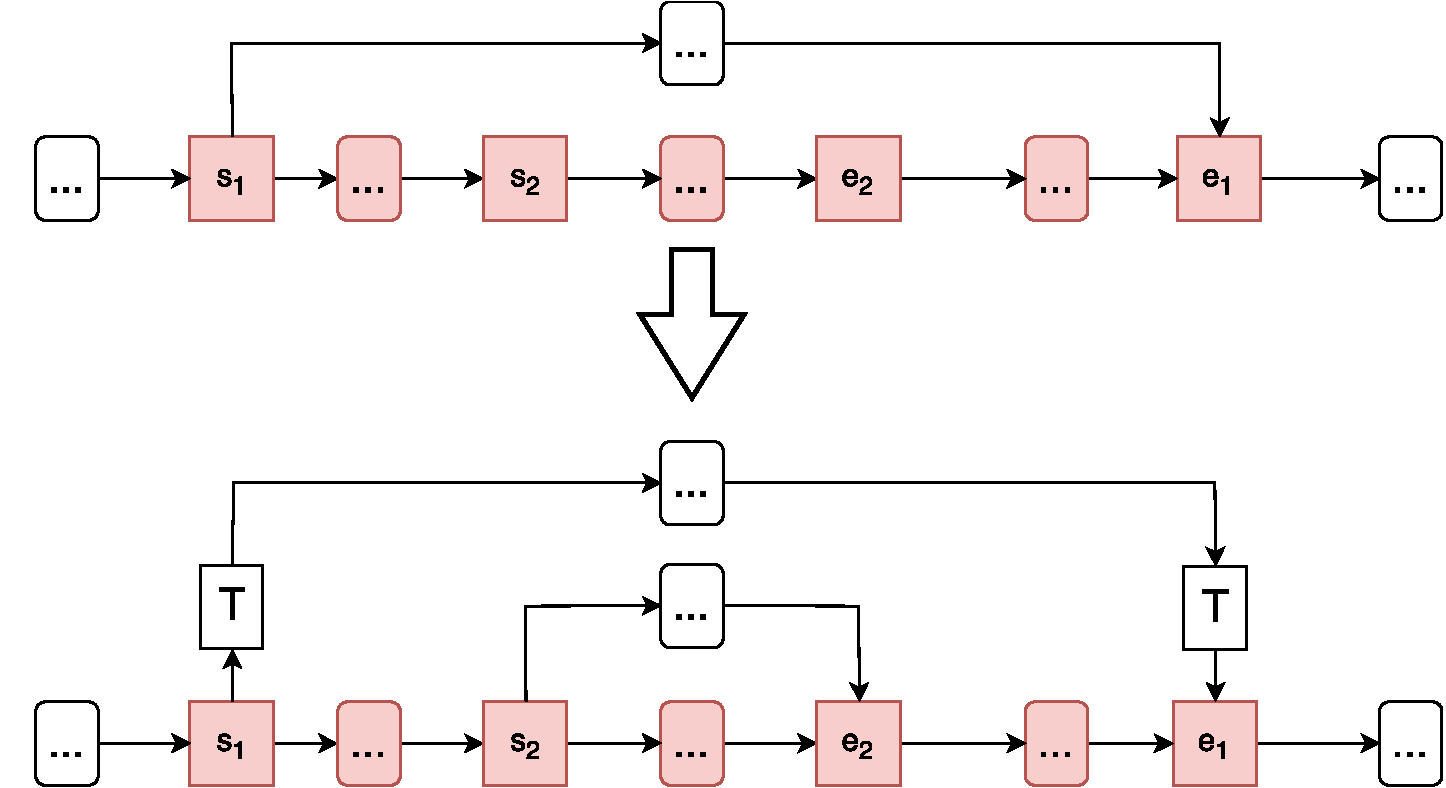
\includegraphics[width=\textwidth]{conflict3.pdf}
\caption{How push underneath handles the case, where we insert a new line that is covered entirely by an old line}
\label{fig:pushunderneath1}
\end{figure}

In the case where the new line covers the old, we handle intersection as in \cref{fig:pushunderneah2}. As we push up the new line we need to push up the old. However, we need not use transport modules to reconnect the old line, instead it can be reached by flowing vertically through the new line.

Again the cases where there is a partial intersection between old and new line is easy to imagine. If the moving up of an old line creates a new intersection, we just move up the line that was already set in place. This is done until no more intersections occur. When this has been done, some old lines may have been disconnected from their main line. We handle this by allowing items to reach them by moving vertically through existing modules and appending transport modules when needed.  

As can be seen, push underneath functions in a manner opposite to push around. We decide to use it when handling intersections that occur as a result of a parallel transformation. We want our parallel lines to be close to the line, which it sprouted from, otherwise we may not reap the benefits of adding extra modules. This is not needed as much, when doing anti-serialization, which is why we use push around for that instead.

  

\begin{figure}[H]
\centering
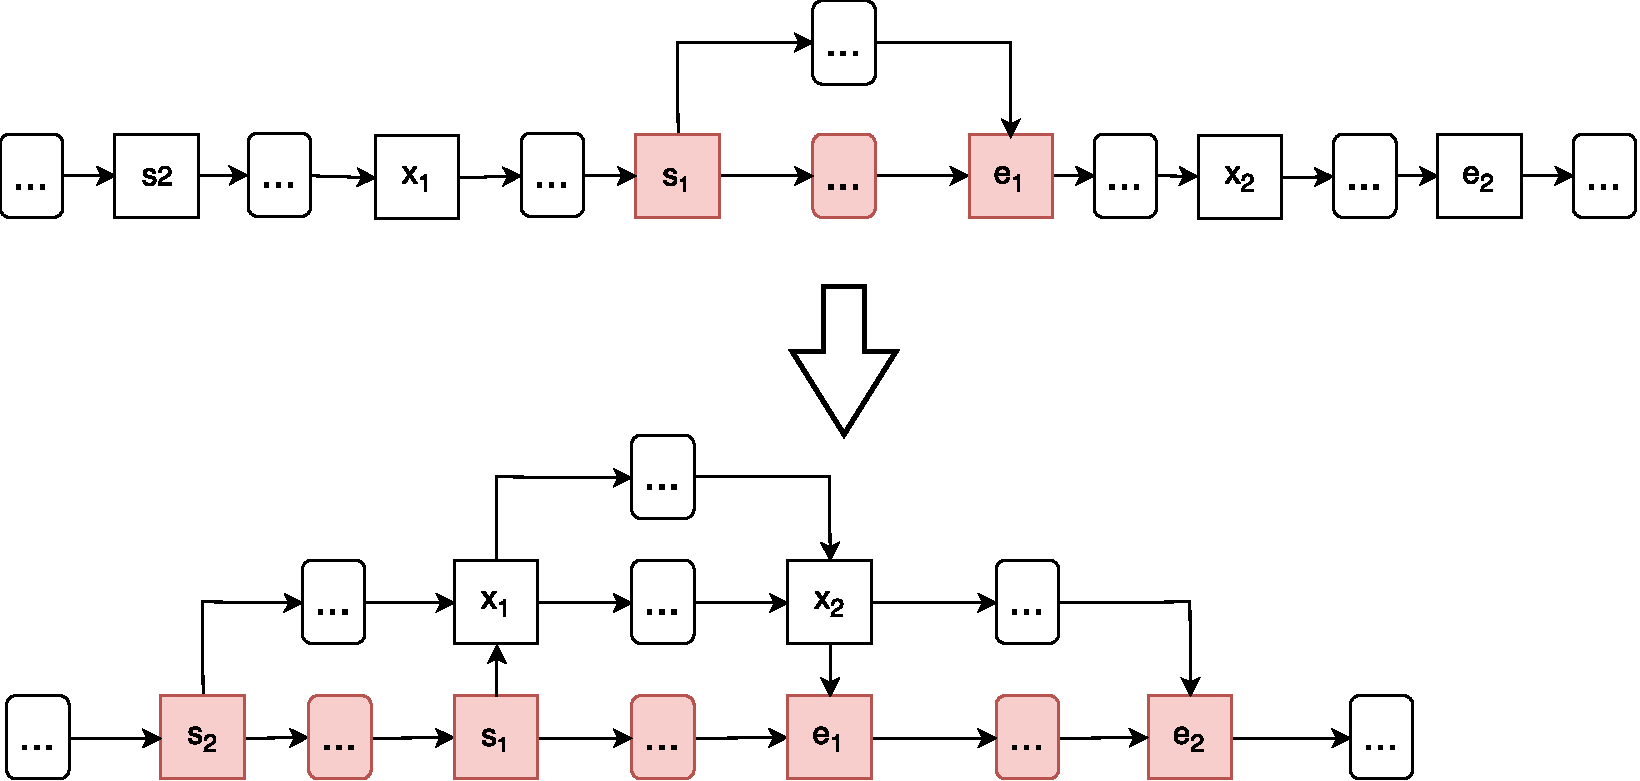
\includegraphics[width=\textwidth]{conflict4.pdf}
\caption{How push underneath handles the case, where we insert a new line that  entirely covers an an old line}
\label{fig:pushunderneath2}
\end{figure}

